% Chapter 5

\chapter{IMPLEMENTATION} % Write in your own chapter title
This chapter will discuss in detail how Off-the-hook-plus is implemented along with the key results and snapshots for better understanding.

\section{ADD-ON}
The add-on has the following components that were implemented using javascript and php as a Google Chrome extension.

\subsection{CONTENT SCRIPT}
This component takes the input which is the URL of the page and it’s contents and sends it to the background process along with the redirection URL from the background script. A design of this component is required as the Chrome Extension cannot get the tab HTML content in the background and so a script in PHP is used to get the content of the URL from the Javascript code segment. Figure ~\ref{fig:contentscript} shows the content script.\\
\null\quad\textit{tablink = tab.url;}\\
\null\quad\textit{\$html = file\_get\_contents(\$site);}\\

\begin{figure}[htp]
\centering
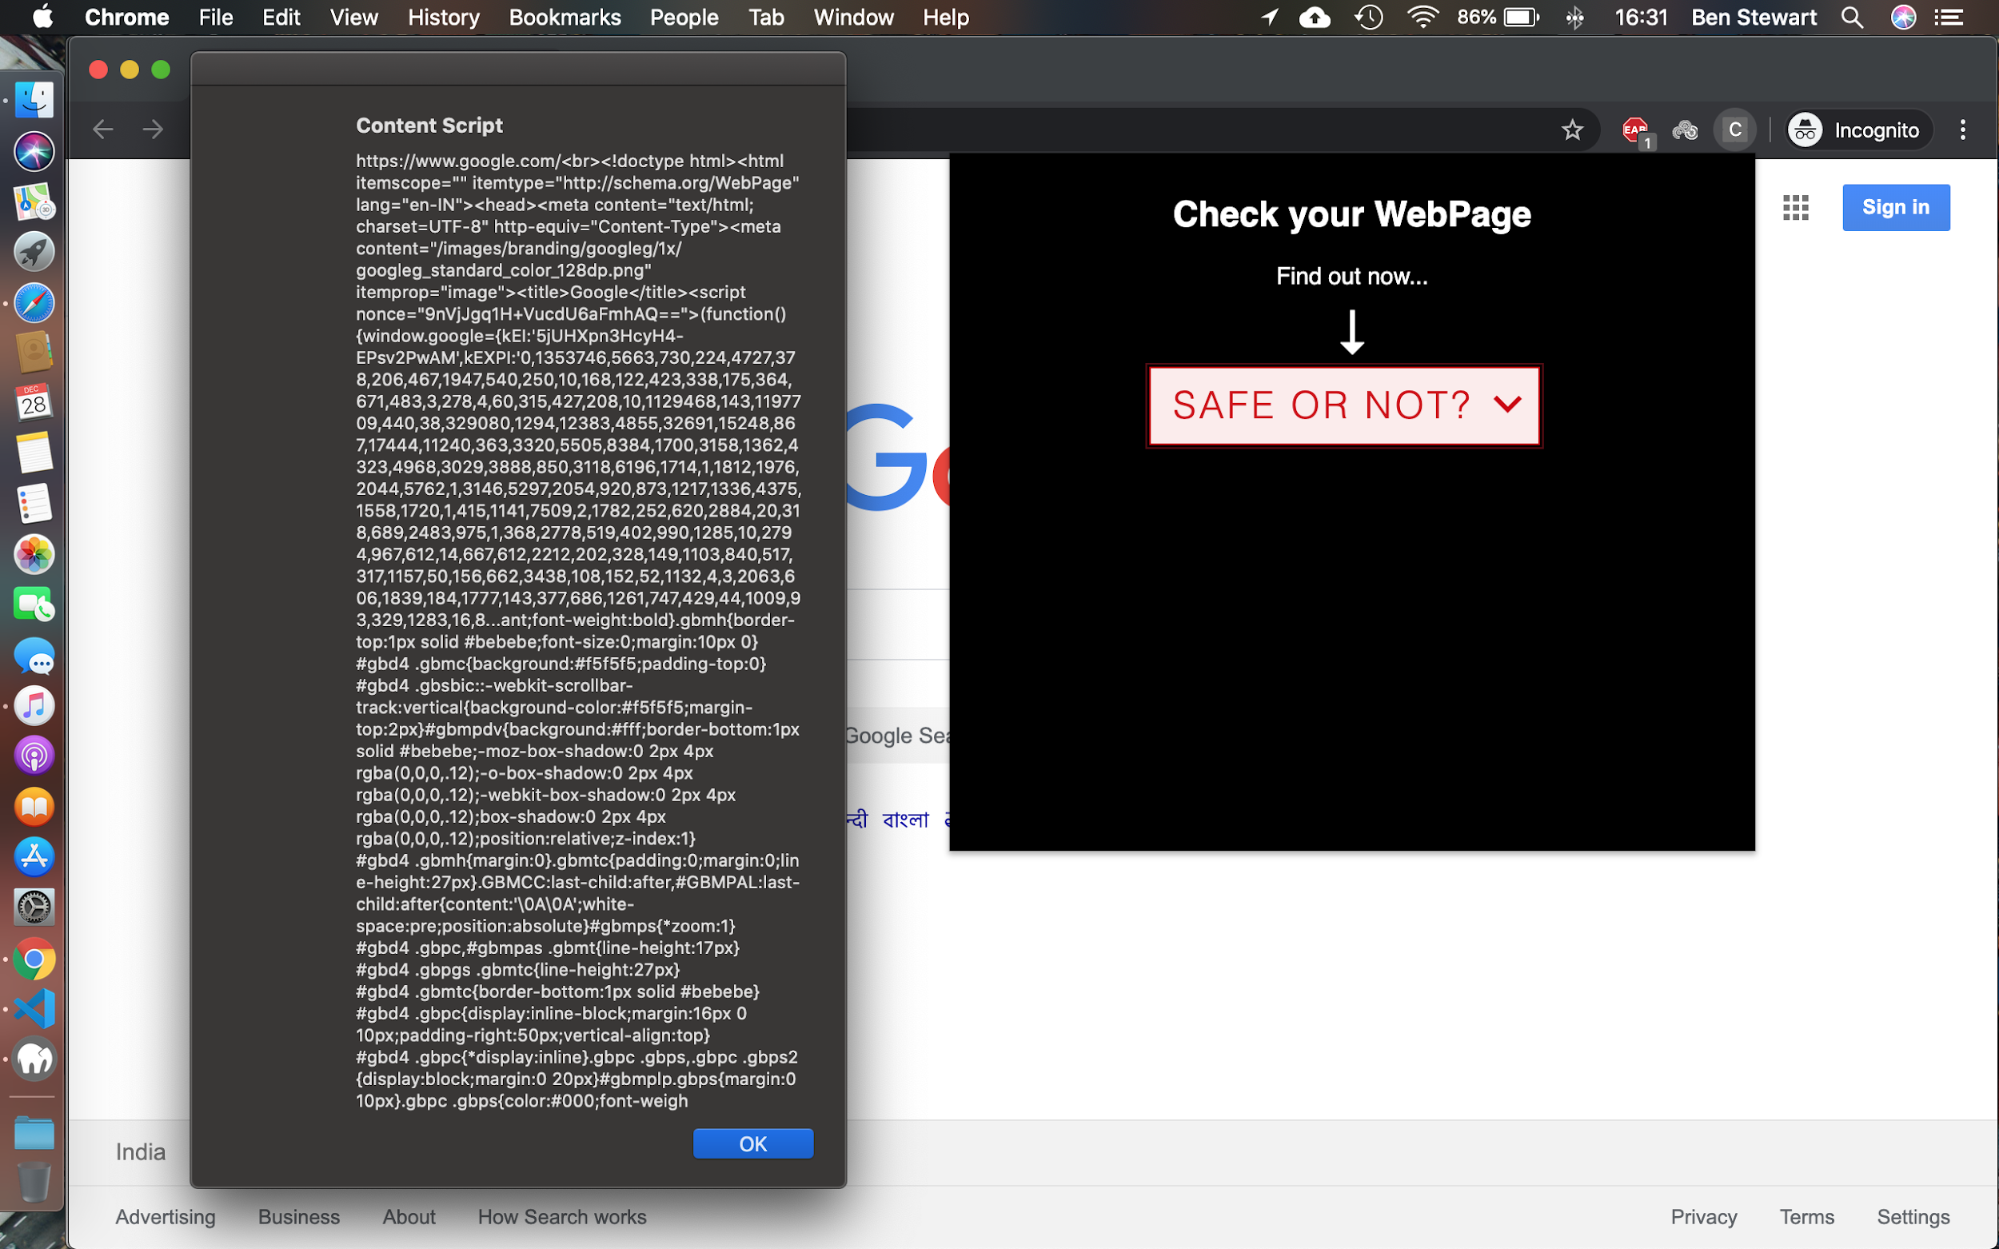
\includegraphics[scale=0.15]{Figures/image9.png}
\caption{Content Script}
\label{fig:contentscript}
\end{figure}

\subsection{BACKGROUND SCRIPT}
This script is based on the open sourced code on GitHub\cite{ccampbell} that demos how to get the background URL redirects of the current tab. It handles multiple types of redirects and also their security levels based on the URL redirects. This component finally returns the list of path components that the page had traversed through. Figure ~\ref{fig:bgscript} shows the background script contents. It has the path items, which are,


\begin{enumerate}
    \item URL
    \item Status
    \item Redirect type
    \item Meta timer
 \end{enumerate}

\begin{figure}[htp]
\centering
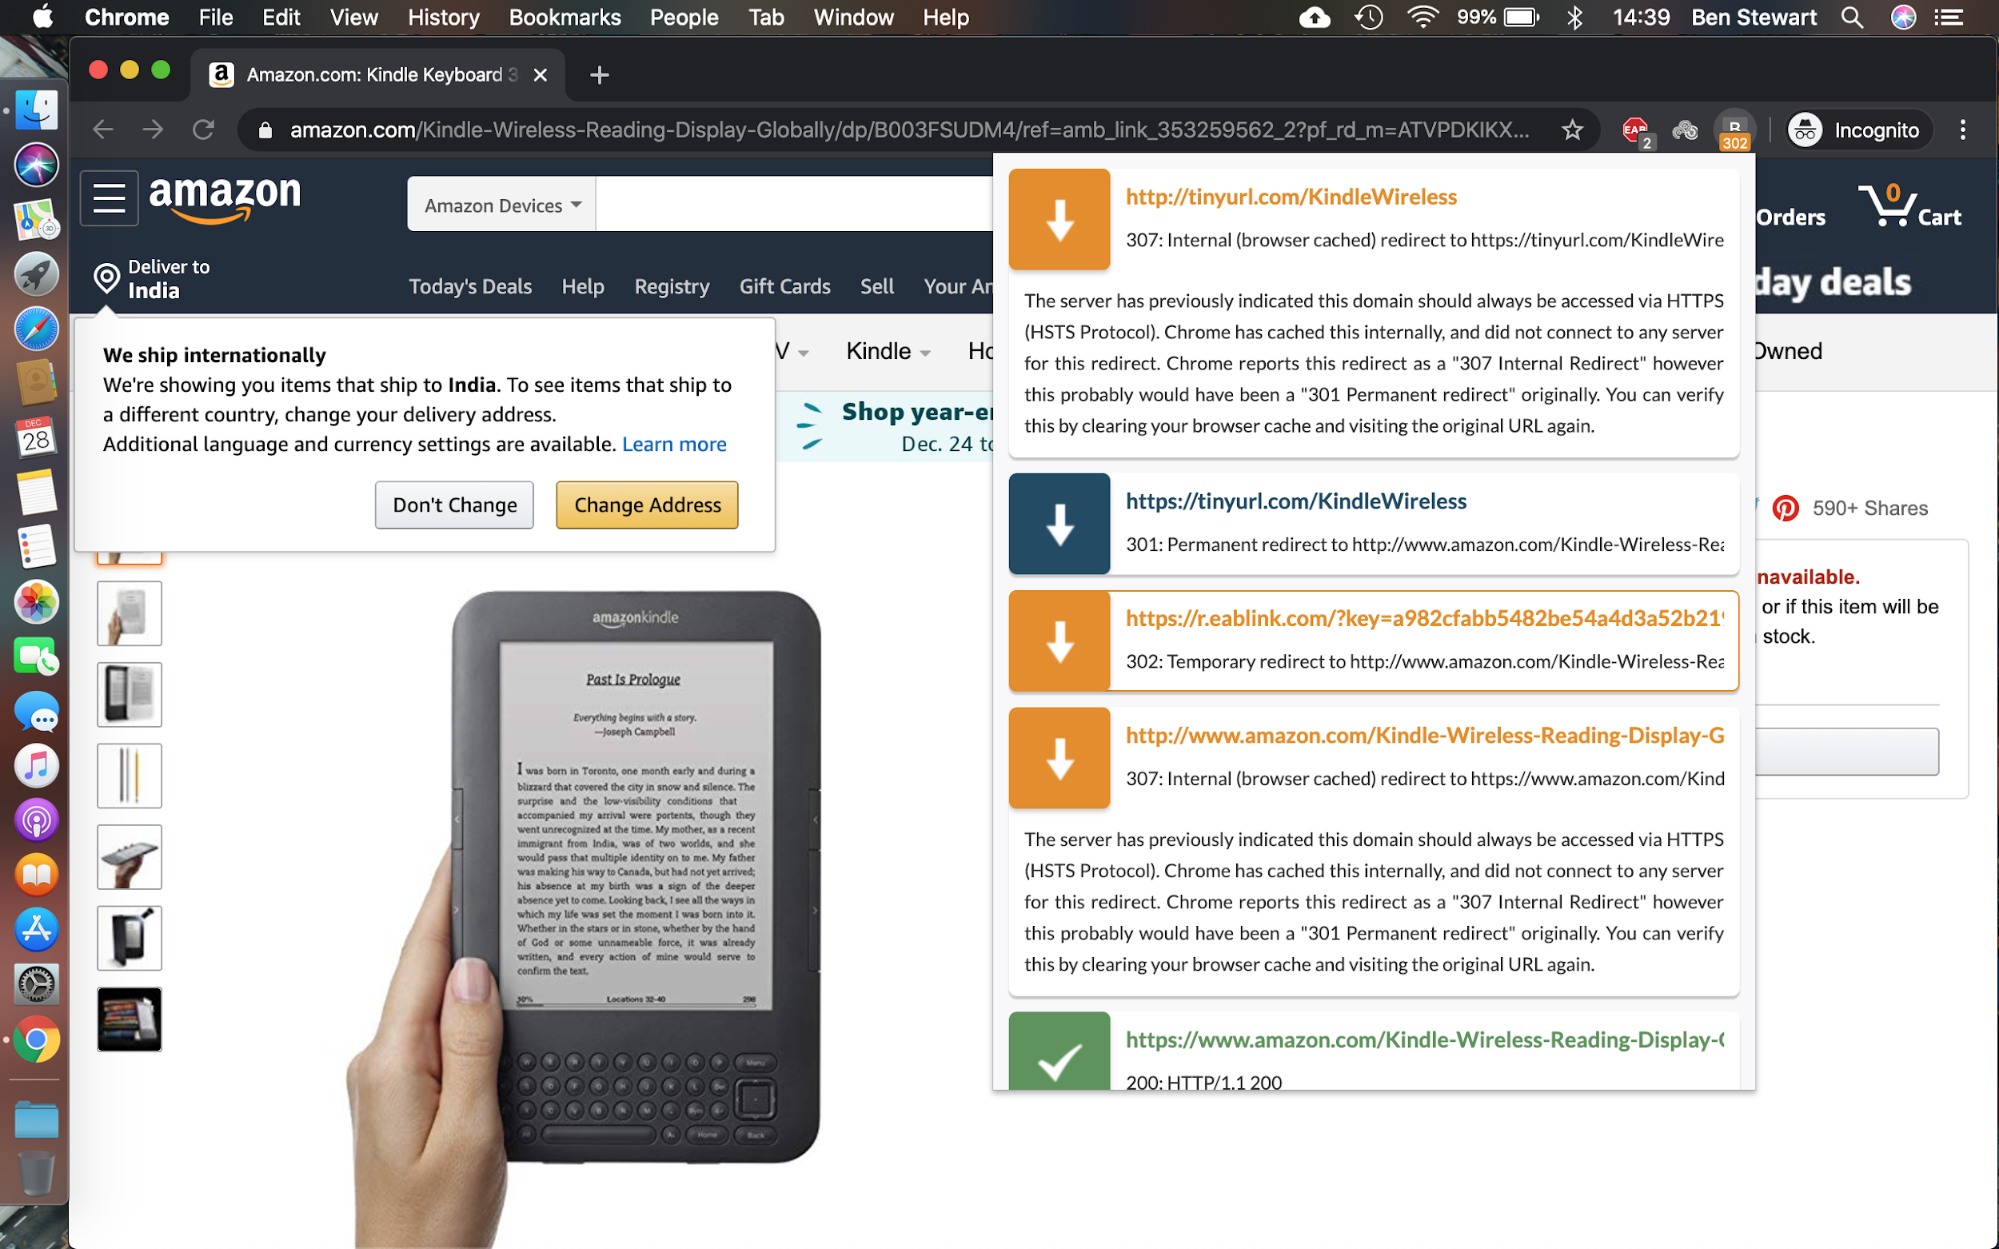
\includegraphics[scale=0.15]{Figures/image5.png}
\caption{Background Script}
\label{fig:bgscript}
\end{figure}

\section{BACKGROUND PROCESS}
This component receives the data from the add-on and orchestrates the decision making using the dispatcher.

\subsection{PHISH DETECTOR}
The dataset used for this project was scraped from PhishTank\cite{pt} and has the records for 23827 such phishing sites with 30 features for each one of them. As a model using all features will take more time to execute, the most important features have to be extracted.

The phish detector is a random forest model trained using the features derived from the Fuzzy Rough Set Theory for feature selection. A few roadblocks faced while developing this model were that the feature selection kit required the data set to be as integers.

The base component was using the scikit roughsets package available in Python. The code is as follows and the output features were used to train the random forest model and provides the output as shown in Figure ~\ref{fig:featureselection}.\\
\null\quad\textit{selector = RoughSetsSelector()}\\
\null\quad\textit{X\_selected = selector.fit(X, y).transform(X)}\\

\begin{figure}[htp]
\centering
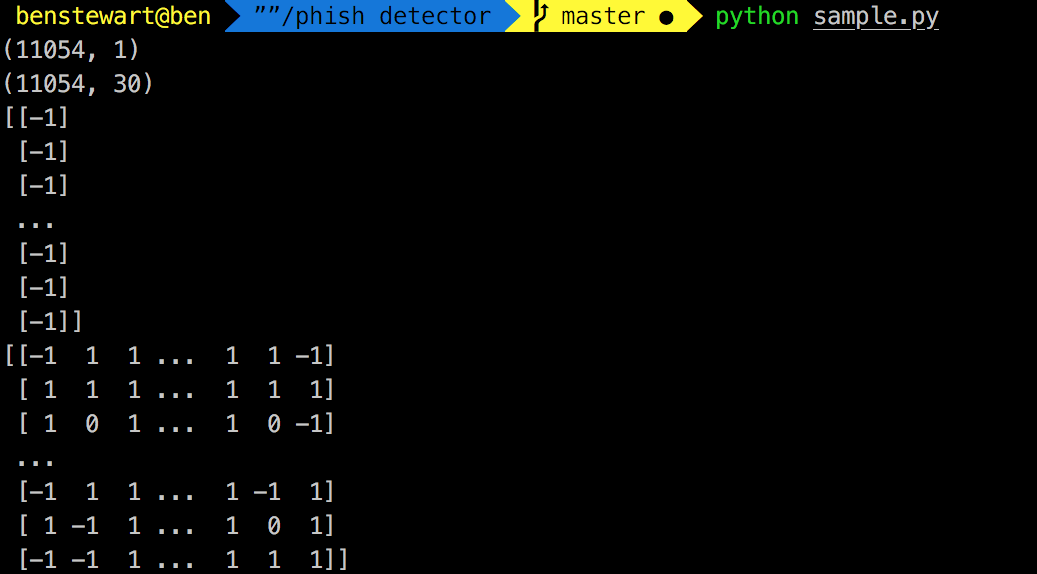
\includegraphics[scale=0.5]{Figures/image16.png}
\caption{Feature Selection}
\label{fig:featureselection}
\end{figure}

The model was generated using the following code and stored as a pickle in the file.\\
\null\quad\textit{//create model}\\
\null\quad\textit{clf4=RandomForestClassifier(min\_samples\_split=7)}\\
\null\quad\textit{clf4.fit(features\_train, labels\_train)}\\
\null\quad\textit{//save the model}\\
\null\quad\textit{joblib.dump(clf4, 'classifier/random\_forest.pkl', compress=9)}\\

Figure  ~\ref{fig:randomforest} gives the confusion matrix and the feature weightage score using the code as follows.\\
\null\quad\textit{//feature weightage}\\
\null\quad\textit{importances = clf4.feature\_importances\_}\\
\null\quad\textit{//confusion matrix}\\
\null\quad\textit{print metrics.confusion\_matrix(labels\_test, pred4)}\\

\begin{figure}[!htp]
\centering
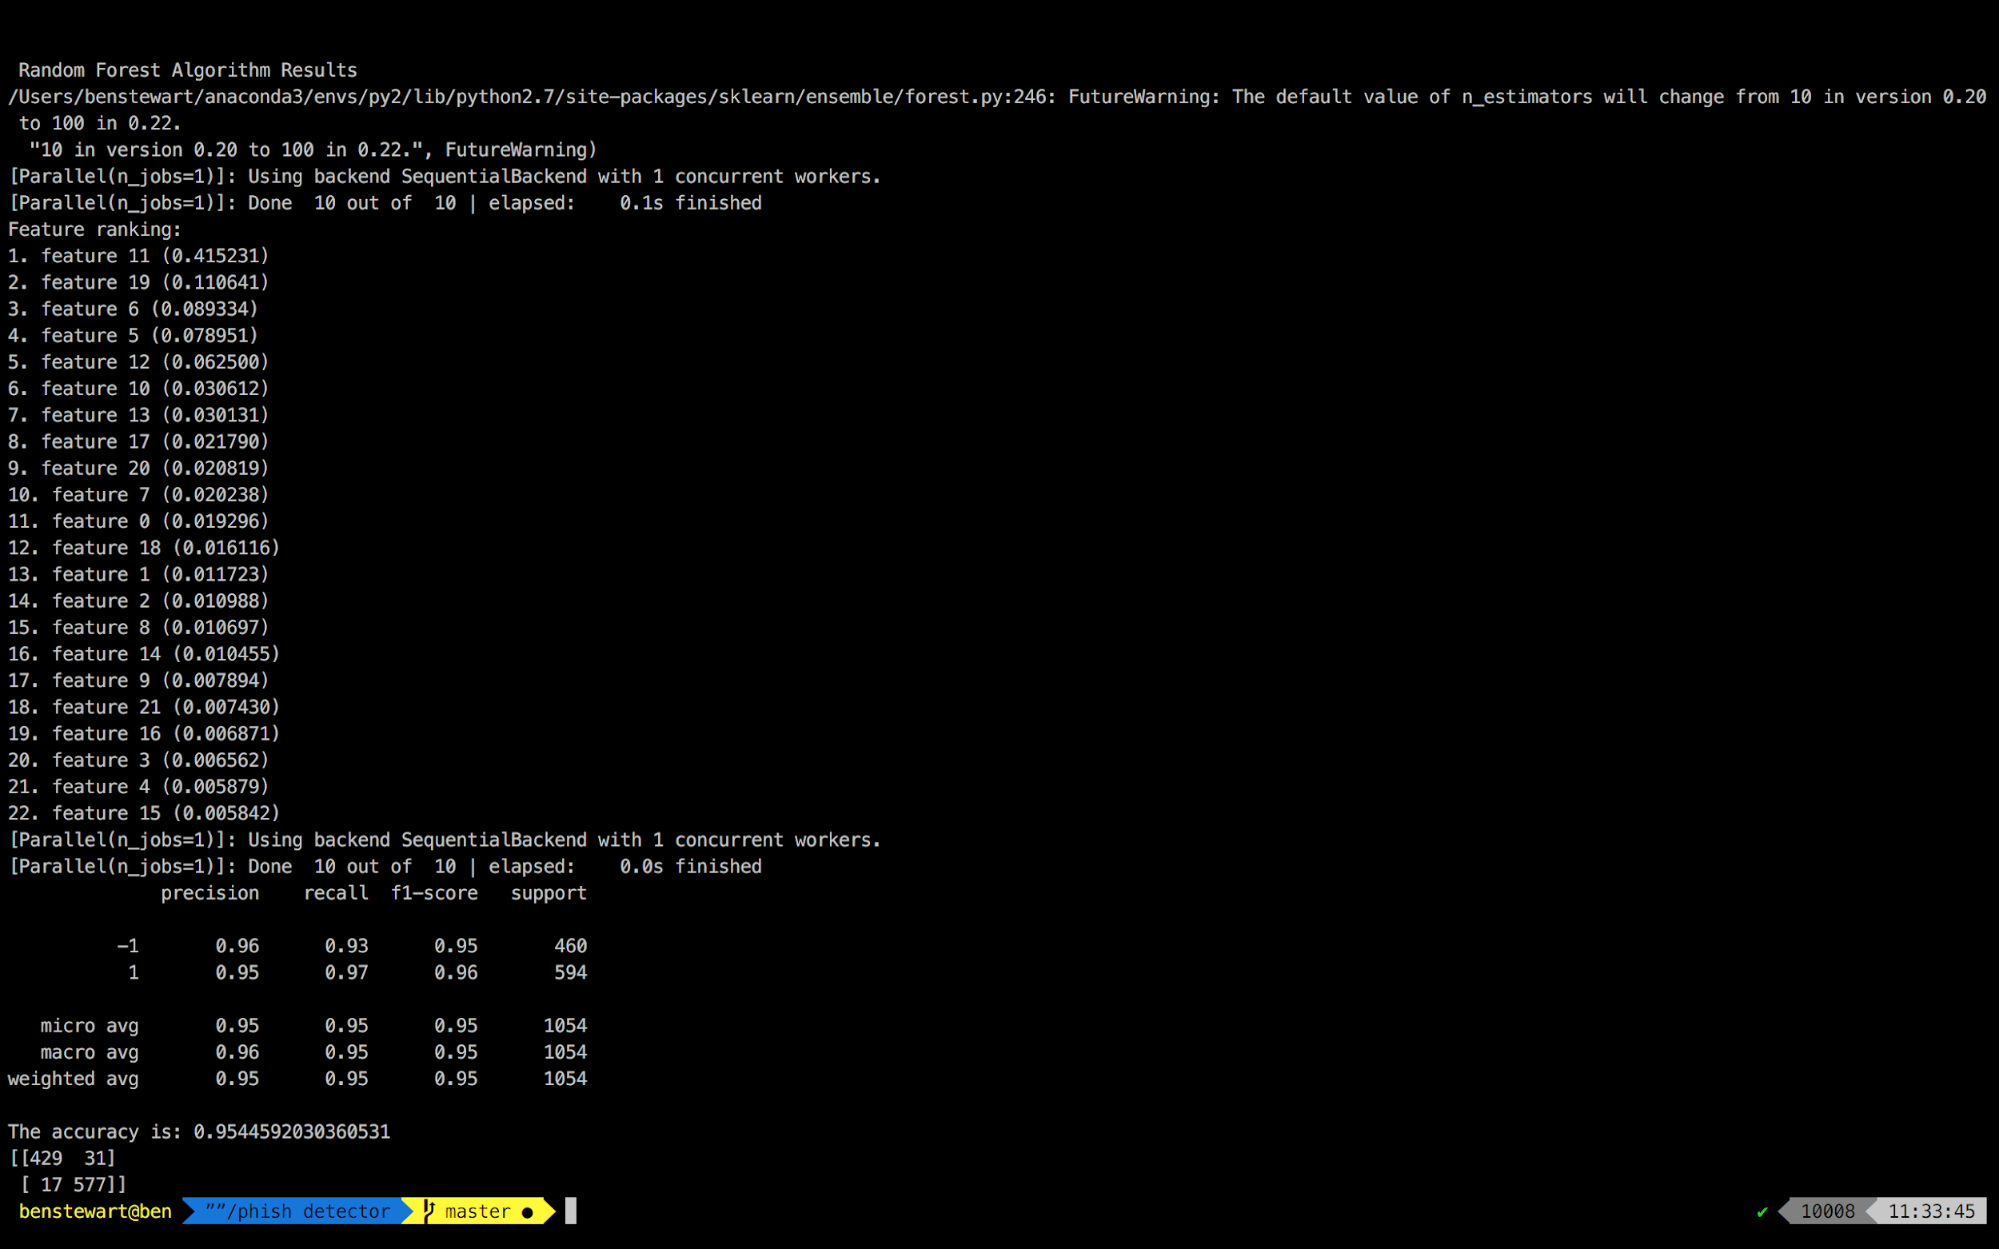
\includegraphics[scale=0.2]{Figures/image7.png}
\caption{Random Forest Model}
\label{fig:randomforest}
\end{figure}

\subsection{TARGET IDENTIFIER}
The target identifier uses the following code to find the similarity between two web pages using the following code.\\
\null\quad\textit{tags1 = get\_tags(lxml.html.parse(path1))}\\
\null\quad\textit{tags2 = get\_tags(lxml.html.parse(path2))}\\
\null\quad\textit{diff = difflib.SequenceMatcher()}\\
\null\quad\textit{diff.set\_seq1(tags1)}\\
\null\quad\textit{ diff.set\_seq2(tags2)}\\

The dispatcher once it confirms that the site is a phish from the phish detector and then writes the url into the single-sites.json file. The url is taken from there and scraped along with the html content and is then compared using the above method.\\
\null\quad\textit{params['url'] = url}\\
\null\quad\textit{response = requests.get(url, headers=headers, params=params)}\\

\subsection{AUTO UPDATED WHITELIST}
The whitelist is automatically updated by the dispatcher if the url is detected to be safe using the following code.\\
\null\quad\textit{//insert into whitelist}\\
\null\quad\textit{white\_list\_file=open('whitelist.txt', "a+")}\\
\null\quad\textit{white\_list\_file.write(url)}\\

The whitelist is searched for before using the ML model to detect if the site is phishing or not, to save execution time.\\
\null\quad\textit{white\_list\_file = open('whitelist.txt').read()}\\
\null\quad\textit{white\_list = white\_list\_file.split('\\n')}\\
\null\quad\textit{if url in white\_list:}\\
\null\quad\textit{\#url is safe}\\

Figure  ~\ref{fig:etauw} gives the shortening of execution time as the url is stored in the whitelist.

\begin{figure}[htp]
\centering
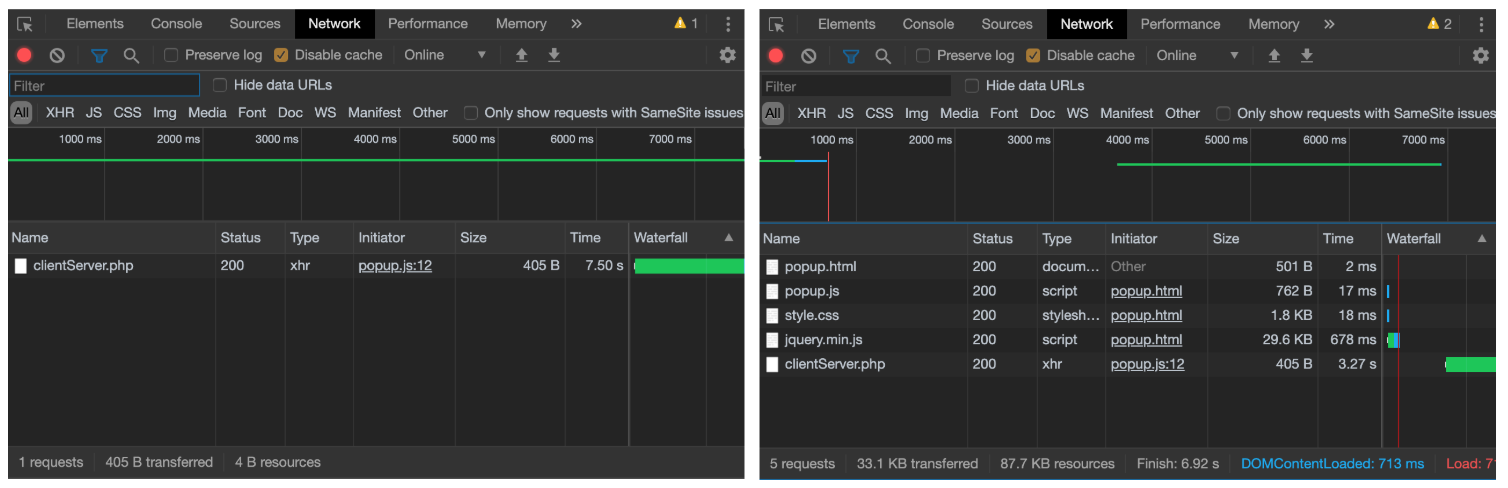
\includegraphics[scale=0.5]{Figures/image12.png}
\caption{Execution Time with Auto Updated Whitelist}
\label{fig:etauw}
\end{figure}

\subsection{DISPATCHER}
The dispatcher is called using the php script of the content script using the following statement.\\
\null\quad\textit{\$decision=exec("python test.py \$site 2$>$\&1 ");}\\
\null\quad\textit{echo \$decision;}\\

The command is run in the default shell of the machine and the output is passed to the Output UI of the add-on that reflects the same in the web browser.

\section{WEB BROWSER}
This component is what takes care of how and what is displayed to the end user when the application is being used.

\subsection{OUTPUT UI}
The content from the dispatcher is loaded into the Google Chrome Extension using the Output UI which has the content loaded into the div that has the HTML, JS and CSS designed for it upfront as shown in the Figure ~\ref{fig:oui}.\\
\null\quad\textit{\$("\#div1").text(xhr.responseText);}\\

\begin{figure}[htp]
\centering
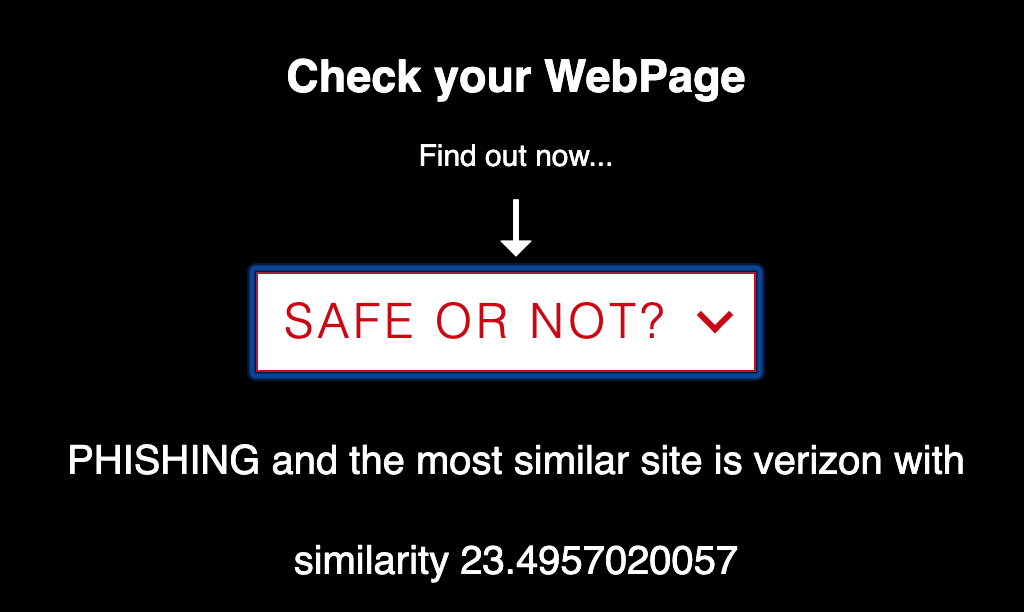
\includegraphics[scale=0.5]{Figures/image13.png}
\caption{Output UI}
\label{fig:oui}
\end{figure}

\subsection{HTML CONTENT}
The web browser must also take care of the whole extension so that the components do not get hidden and also are not visible to the user. The following css snippet makes sure the above holds good as shown in the Figure ~\ref{fig:htmlc}.\\
\null\quad\textit{body\{}\\
\null\quad\quad\textit{width:500px;}\\
\null\quad\quad\textit{height:100px;}\\
\null\quad\quad\textit{display:inline-block;}\\
\null\quad\quad\textit{align-items: center;}\\
\null\quad\textit{\}}\\

\begin{figure}[htp]
\centering
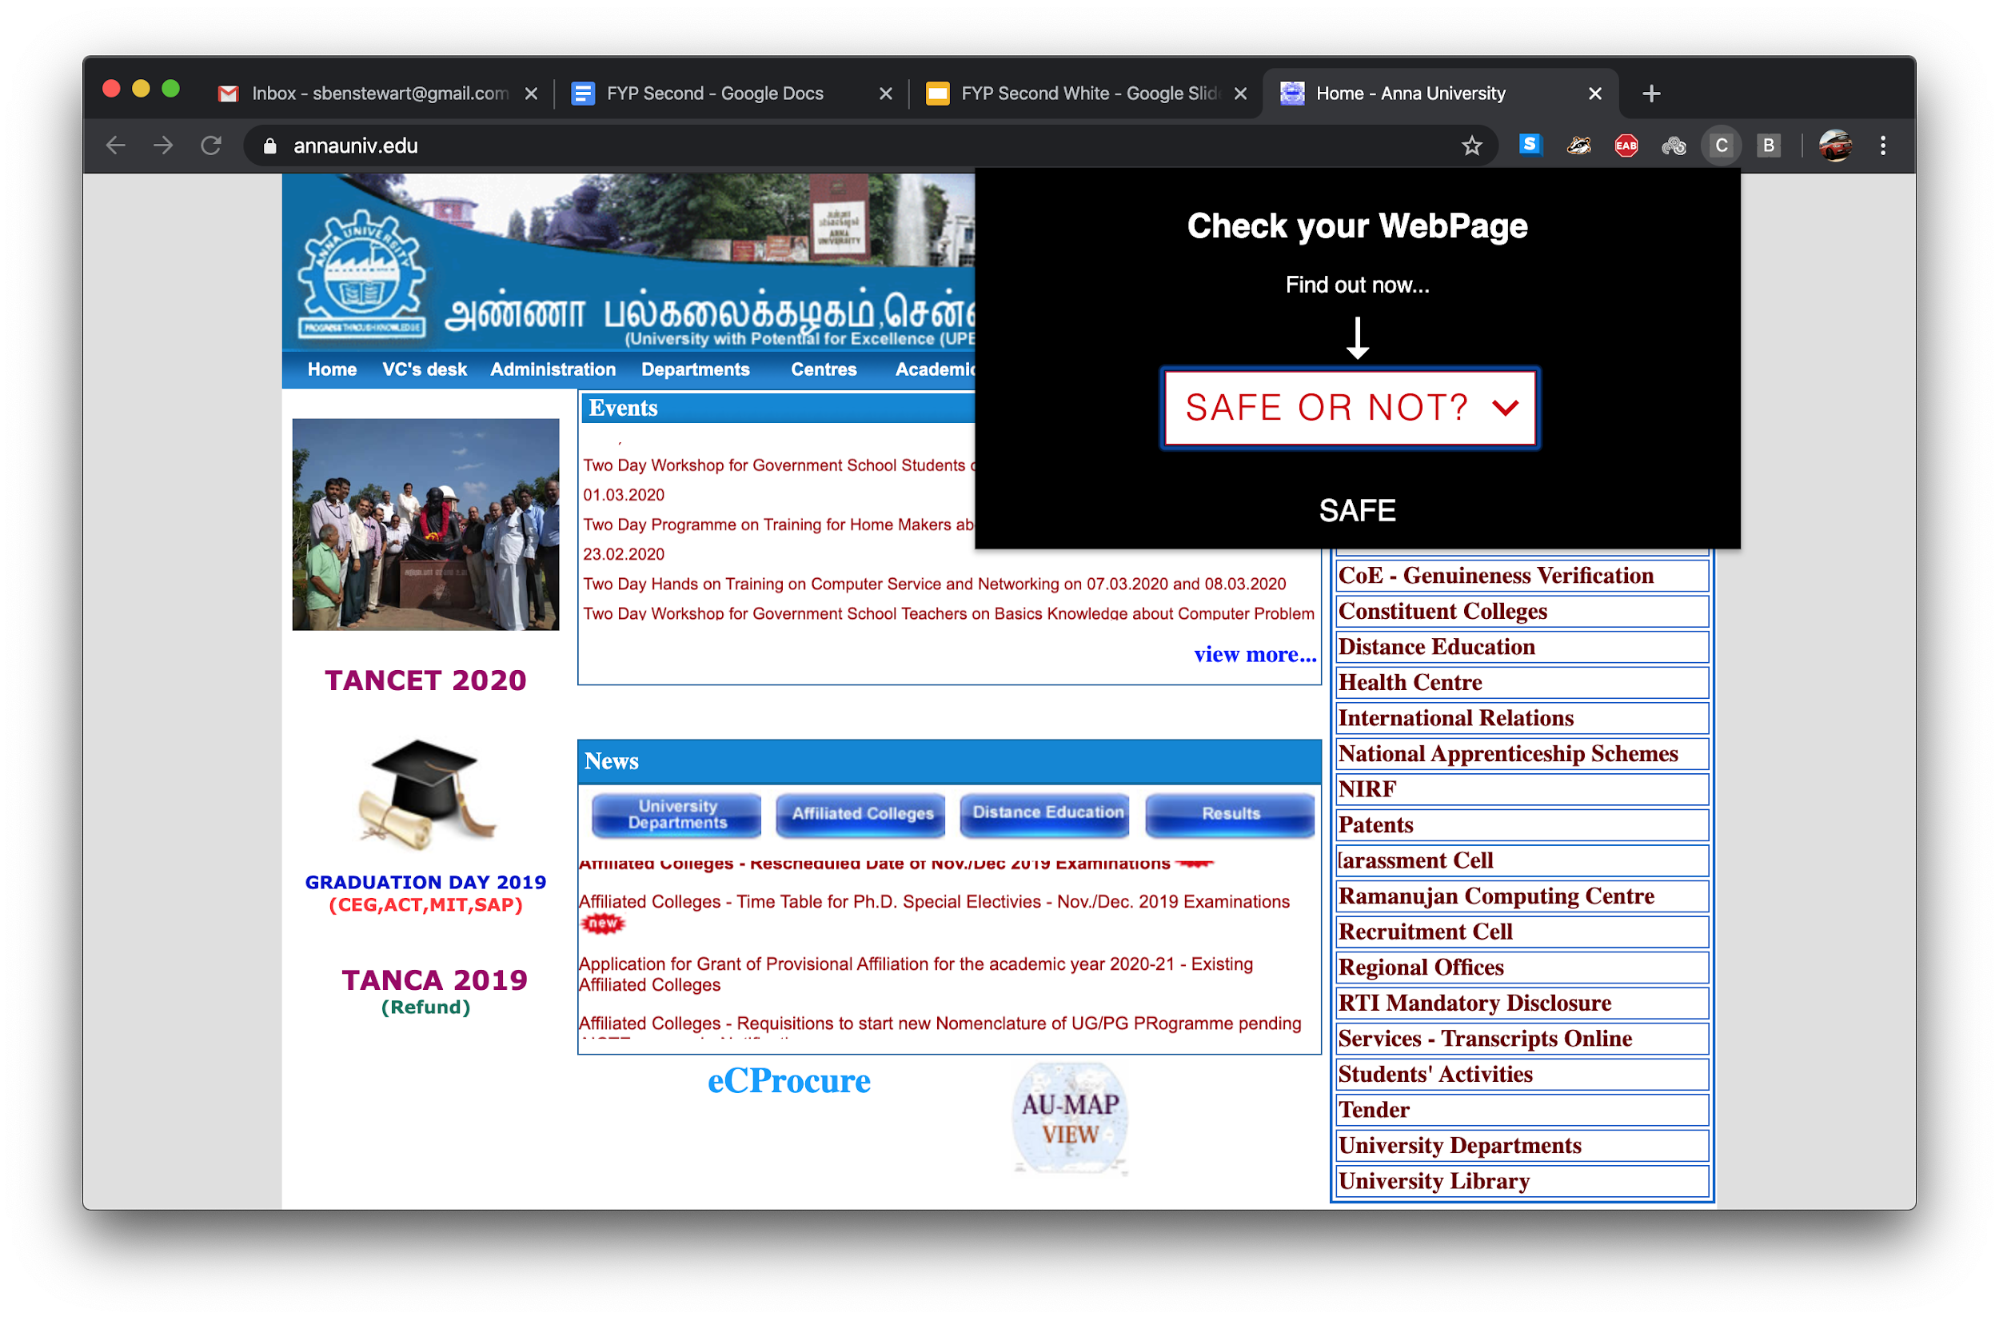
\includegraphics[scale=0.2]{Figures/image2.png}
\caption{HTML Content}
\label{fig:htmlc}
\end{figure}


















